\documentclass[aspectratio=1610,compress,t,gabaritb,french,english]{hecppt}

%% Packages
\usepackage{fontawesome}
\usepackage{metalogo}
\usepackage{listings}
\usepackage{tabularx}
\usepackage{colortbl}
\usepackage{makecell}
\usepackage{hyperref}

%% Commandes
\newcommand{\cmd}[1]{%
	\texttt{\textbackslash #1}
}

\newcommand{\lien}[2]{%
	\href{#1}{#2 \faExternalLink}
}

%% Environnements
\lstnewenvironment{codesource}{%
	\lstset{%
		basicstyle=\tiny,
		language=[LaTeX]TeX,
		backgroundcolor=\color{bleuPaleSecondaire!10},
		tabsize=2,
		% frame=leftline,
		% numbers=left,
		% numberstyle=\tiny,
		literate=%
		{à}{{\`a}}1
		{é}{{\'e}}1
		{ç}{{\c c}}1
		{«}{{\og}}1
		{»}{{\fg}}1
	}
}{}

%% Options des packages
\hypersetup{colorlinks=true,%
	urlcolor=bleuFoncePrimaire,%
	linkcolor=bleuFoncePrimaire,%
	pdfauthor=Benoit Hamel,%
	pdftitle=Rédaction avec LaTeX : Principes de base}
\frenchbsetup{og=«,fg=»}
\setlength{\parskip}{1ex}
\renewcommand{\cellalign}{tl}

%% Métadonnées du document

\title{Writing with \\ \texttt{\textbackslash title}\{\textrm{\LaTeX}\} }
\subtitle{The Basics}
\HECauteur{Benoit Hamel}{Benoit Hamel}
\date[2018-02-28]{2018-02-28}
\subject{} % Sujet inséré dans les métadonnées du pdf
\keywords{} % Mots-clés insérés dans les métadonnées du pdf

\begin{document}

\pageTitre

% Pages liminaires
\scriptsize

% Page titre
\begin{frame}
	Benoit Hamel \\
	Technicien en documentation, soutien technique \\
	Bibliothèque HEC Montréal
	\vfill
	{
		\Huge\bfseries
		Rédaction avec \\
		\texttt{\textbackslash title\{\textrm{\LaTeX}\}}
	}
	\vfill
	Première partie : Principes de base \\
	Édition HEC Montréal, revue et augmentée (version française)
\end{frame}

% Page de la licence
\begin{frame}
	\faCopyright\ 2016 Vincent Goulet pour la 
	\href{https://ctan.org/pkg/formation-latex-ul}{version originale}. La liste des sources qui ont 
	servi à l'élaboration de cette formation se trouve à la fin du présent document.
	
	\faCreativeCommons\ Cette création est mise à disposition selon le contrat 
	\href{http://creativecommons.org/licenses/by-sa/4.0/deed.fr}{%
	Attribution-Partage dans les mêmes conditions 4.0 International de Creative Commons}. 
	En vertu de ce contrat, vous êtes libre de :
	
	\begin{itemize}
		\item partager -- reproduire, distribuer et communiquer l’oeuvre;
		\item remixer -- adapter l’oeuvre;
		\item utiliser cette oeuvre à des fins commerciales.
	\end{itemize}

	Selon les conditions suivantes :
	
	\begin{itemize}
		\item Attribution -- Vous devez créditer l’oeuvre, intégrer un lien vers le contrat et indiquer si des modifications ont été effectuées à l’oeuvre. Vous devez indiquer ces informations par tous les moyens possibles, mais vous ne pouvez suggérer que l’Offrant vous soutient ou soutient la façon dont vous avez utilisé son oeuvre.
		\item Partage dans les mêmes conditions -- Dans le cas où vous modifiez, transformez ou créez à partir du matériel composant l’oeuvre
		originale, vous devez diffuser l’oeuvre modifiée dans les même conditions, c’est-à-dire avec le même contrat avec lequel l’oeuvre originale a été diffusée.
	\end{itemize}
\end{frame}

% Table des matières
\begin{frame}{Sommaire de la formation}
	\begin{columns}[onlytextwidth]
		\begin{column}{.49\textwidth}
			\tableofcontents[sections={1-3}]
		\end{column}
		\begin{column}{.49\textwidth}
			\tableofcontents[sections={4-6}]
		\end{column}
	\end{columns}
\end{frame}
% Présentation de TeX et LaTeX
\small

\section{\TeX\ and \LaTeX\ presentation}

\subsection{What is \TeX\ and \LaTeX?}

\begin{frame}[c,label=fr:commencement]{At the beginning (1978), there was \TeX\ldots}
	
\includegraphics[width=\textwidth,keepaspectratio=true]{knuth-tex-commencement.jpg}
\end{frame}

\begin{frame}[c]{What is \TeX?}

	\begin{itemize}
		\item A typesetting and document preparation system;
		\item ``The most powerful formatting program for producing book-quality text 
			of scientific and technical works''\footnote{Kopka \& Daly, p. 6};
		\item A mature, stable, complete and bug-free system;
		\item A set of very primitive commands perfect for typography and
			programming functions;
		\item «\emph{typesetter-level program}».
	\end{itemize}

\end{frame}

\begin{frame}[c,label=fr:sixiemejour]{On the sixth day (1983), there was \LaTeX\ldots}
	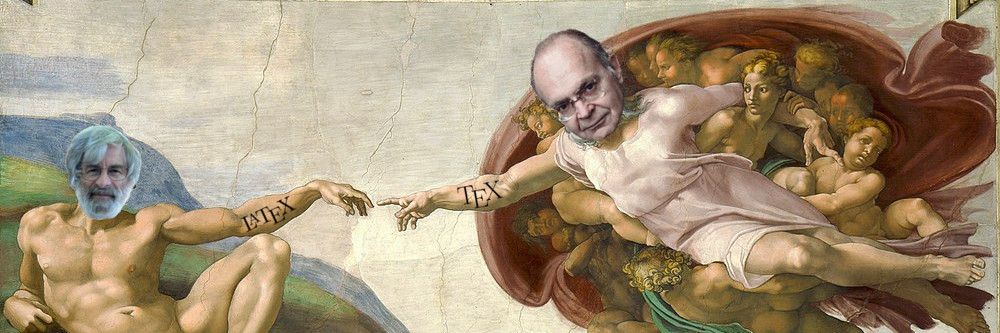
\includegraphics[width=\textwidth,keepaspectratio=true]{creation-of-latex.jpg}
\end{frame}

\begin{frame}{What is \LaTeX?}
	\begin{itemize}
		\item A set of macro-commands used to facilitate \TeX's usage;
		\item No preliminary knowledge of typography in general or \TeX\ in particular
			is required;
		\item Typographical and logical markup language used for text layout (like HTML);
		\item Cross-platform language, identical from one operating system to the other,
			and extensible with packages;
		\item «\emph{author-level program}».
	\end{itemize}
\end{frame}

\subsection{A \LaTeX\ document creation process}

% Rédiger avec une nouvelle perspective
\begin{frame}[c]{Writing with a new perspective}
	
	\begin{itemize}
		\item You write your document in plain text and use commands to describe
			\textbf{what your text is} and \textbf{not what it's supposed to look like}.
		\item You concentrate on your \textbf{content}.
		\item You let \LaTeX\ do its work, that is taking care of the \textbf{container}.
	\end{itemize}
	
\end{frame}

% Processus de création d'un document LaTeX
\begin{frame}[c]{\LaTeX\ document creation process}
	\Huge
	\begin{minipage}[t]{0.25\linewidth}
		\centering
		\faFileTextO
	\end{minipage}
	\hfill\faArrowRight\hfill
	\begin{minipage}[t]{0.25\linewidth}
		\centering
		\faCogs
	\end{minipage}
	\hfill\faArrowRight\hfill
	\begin{minipage}[t]{0.25\linewidth}
		\centering
		\faFilePdfO
	\end{minipage}

	\begin{picture}(0,0)
		\footnotesize\thicklines\color{bleuFonceSecondaire}
		\onslide<2>\put(0,-10){\dashbox{1}(35,40)[b]{\parbox{.2\textwidth}{\centering\textbf{text writing and markup in a text editor\smallskip}}}}
		\onslide<3>\put(54,-10){\dashbox{1}(35,40)[b]{\parbox{.2\textwidth}{\centering\textbf{compilation with a \TeX\ engine from the command line\smallskip}}}}
		\onslide<4>\put(108,-10){\dashbox{1}(35,40)[b]{\parbox{.2\textwidth}{\centering\textbf{visualization with an external viewer\smallskip}}}}
	\end{picture}
\end{frame}
% Création d'un document LaTeX

\section{\LaTeX\ document creation}

\subsection{Document structure}

% Un document LaTeX dans sa plus simple expression
\begin{frame}[c,fragile]{The most basic \LaTeX\ document}

	In a text editor, open a new file and write the following code:
	
\begin{codesource}	
	\documentclass{article}
	
	\begin{document}		
		This is my first LaTeX document and I am proud of it.
	\end{document}

\end{codesource}

	Save your file with the \texttt{.tex} extension and compile it. Look at the results.
	
\end{frame}

% Les parties d'un document : la déclaration de la classe de document
\begin{frame}[c,fragile]{The parts of a document}
	\framesubtitle{Document class declaration}
	\begin{itemize}
		\item A document always starts with the \cmd{documentclass} \textbf{command}.
		
\begin{codesource}
	\documentclass[options]{class}
\end{codesource}

		\item The \lien{https://en.wikibooks.org/wiki/LaTeX/Document_Structure\#Document_classes}{document class}
			determines a document's type.		
		\item Many options can be used to change a document's layout.
	\end{itemize}
\end{frame}

% Les parties d'un document : le corps du document
\begin{frame}[c,fragile]{The parts of a document}
	\framesubtitle{Document body}
	A document's content is written inside the \texttt{document} \textbf{environment},
	between the \cmd{begin\{document\}} and \cmd{end\{document\}} commands.
\begin{codesource}
	\documentclass[options]{class}
	
	\begin{document}
		The document's content is written here...
	\end{document}
\end{codesource}
\end{frame}

% Les parties d'un document : le préambule
\begin{frame}[c,fragile]{The parts of a document}
	\framesubtitle{The preamble}
	Everything that is written before the \cmd{begin\{document\}} command is called
	the document \textbf{preamble}.
	
\begin{codesource}
	\documentclass[options]{class}
	
	%% Here lies the document preamble...
	
	\begin{document}
		The document's content is written here...
	\end{document}
\end{codesource}

	In the preamble, you will find:
	\begin{itemize}
		\item packages;
		\item configuration commands;
		\item custom commands and environments;
		\item metadata.
	\end{itemize}
\end{frame}

% Création d'un document plus complexe
\begin{frame}[c]{Creating a more complex document}
	\begin{itemize}
		\item Open the first \texttt{.tex} file you created.
		\item Go to the \lien{http://www.hec.ca/en/news/index.html}{HEC Montréal news web page}.
		\item Copy and paste a whole article in your document.
		\item Save and compile your document, then look at the results.
	\end{itemize}
\end{frame}

\subsection{\LaTeX\ customization}

% Préambule : les packages
\begin{frame}[fragile,c]{Preamble}
	\framesubtitle{Packages}
	Packages are used to \textbf{modify commands} or \textbf{add functionalities} to the system.
	
	They are loaded in the preamble with the \cmd{usepackage[options]\{package\}} command.

\begin{codesource}
	\documentclass[options]{class}
	
	\usepackage{package}
	\usepackage[options]{package}
	\usepackage{package1,package2,package3,...}
\end{codesource}
	
	Each package's documentation can be found on the 
	\lien{https://ctan.org/}{Comprehensive \TeX\ Archive Network} website.
\end{frame}

% Commandes
\begin{frame}[fragile]{Commands}
	\begin{itemize}
		\item Always start with a \textbackslash
		\item General syntax:
\begin{codesource}
	\nomcommande[optional_args]{mandatory_args}
	\nomcommande*[optional_args]{optional_args}
	\nomcommande
\end{codesource}
		\item Mandatory arguments are placed between \{\ and \}
		\item Optional arguments are placed between [ et ]
		\item Commands without arguments : their name ends with any character that isn't a letter, including
			a white space
		\item The scope of a command is limited in the zone between \{\ and \}.
	\end{itemize}
\end{frame}

% Environnements
\begin{frame}[fragile,c]{Environments}
	\begin{itemize}
		\item Delimited by
\begin{codesource}
	\begin{environment}
		...
	\end{environment}
\end{codesource}
		\item An environment's content is treated differently from the remainder
			of the text
		\item Changes only apply inside the environment
	\end{itemize}
\end{frame}

% Commandes et environnements personnalisés
\begin{frame}[c]{Custom commands and environments}
	\begin{itemize}
		\item You can \textbf{create} new commands with \cmd{newcommand}.
		\item You can \textbf{modify} existing commands with \cmd{renewcommand}.
		\item You can \textbf{create} new environments with \cmd{newenvironment}.
		\item You can \textbf{modify} existing environments with \cmd{renewenvironment}.
	\end{itemize}
\end{frame}
\section{Writing}

\subsection{Basic formatting}

% Titre, auteur et date du document
\begin{frame}[fragile]{Title, author and date}
	\begin{itemize}
		\item Automatic formatting
\begin{codesource}
	\documentclass{article}
	
	\title{Document title}
	\author{Author name}
	\date{A date}
	
	\begin{document}
		\maketitle
		
		% Document content...
	\end{document}
\end{codesource}
		\item Manual formatting
\begin{codesource}
	\documentclass{article}
	
	\begin{document}
		\begin{titlepage}
			% Title page built manually...
		\end{titlepage}
	\end{document}
\end{codesource}
	\end{itemize}
\end{frame}

% Paragraphes, sauts de lignes et espaces blancs
\begin{frame}[c]{Paragraphs, line breaks and white space}
	\begin{itemize}
		\item \LaTeX\ automatically deletes all extra white spaces.
		\item Line breaks are created with \textbackslash\textbackslash.
		\item There needs to be at least one blank line between paragraphs in
			the code in order to distinguish them in the text.
	\end{itemize}
\end{frame}

% Caractères spéciaux
\begin{frame}{Reserved characters}
	\framesubtitle{\TeX\ reserved characters}
	\begin{description}[\#]
		\item[\#] Argument identifier in commands
		\item[\$] Math mode delimiter
		\item[\&] Column delimiter in tables
		\item[\%] Start of a comment
		\item[\_] Indice (math)
		\item[\textasciicircum] Exponent (math)
		\item[\textasciitilde] No-break space
		\item[\{] Opens a command or environment definition
		\item[\}] Closes a command or environment definition
	\end{description}
	\begin{picture}(0,0)
	\thicklines\color{bleuFonceSecondaire}
	\onslide<2>\put(90,5){\dashbox{1}(53,58){}}
	\onslide<2>\put(97,59){\textbf{\MakeUppercase{To use them:}}}
	\onslide<2>\put(94,55){\parbox[t]{.3\textwidth}{\centering\bfseries\textbackslash \# \\[5pt] %
			\textbackslash \$ \\[5pt] \textbackslash \& \\[5pt] \textbackslash \% \\[5pt] %
			\textbackslash \_ \\[5pt] \textbackslash textasciicircum \\[4pt] %
			\textbackslash textasciitilde \\[4pt] \textbackslash \{ \\[4pt] %
			\textbackslash \} }}
	\end{picture}
\end{frame}

% Caractères spéciaux - la suite
\begin{frame}[fragile]{Reserved characters}
	\framesubtitle{Part deux\ldots}
	\begin{itemize}
		\item Quote marks
			\begin{itemize}
				\item We open english single quotes with (\lstinline|`|)
					and double quotes with (\lstinline|``|). We close them with one
					(\lstinline|'|) or two (\lstinline|''|) apostrophes, depending on the case.
				\item On utilise les chevrons (« et ») pour ouvrir et fermer les guillemets français.
					Il faut cependant inscrire la commande suivante à la fin de notre préambule:
\begin{codesource}
	\frenchbsetup{og=«,fg=»}
\end{codesource}				
			\end{itemize}
		\item On inscrit les traits d'union avec un tiret (\lstinline|-|), les traits demi-cadratins avec deux tirets (\lstinline|--|) et les traits cadratins avec trois tirets (\lstinline|---|).
	\end{itemize}
\end{frame}

% Commentaires
\begin{frame}[c]{Commentaires}
\begin{itemize}
\item Pour se retrouver dans le code (ou des documents longs), il est conseillé 
d'y insérer des commentaires.
\item Ceux-ci commencent toujours avec le symbole \texttt{\%}.
\item Ils s'affichent dans le code, mais pas dans le document final.
\end{itemize}
\end{frame}

\subsection{Apparence du texte}

% Polices de caractères
\begin{frame}[c]{Polices de caractères}
	\begin{itemize}
		\item Par défaut, tous les documents \LaTeX\ utilisent la même police, \textrm{Computer Modern}.
		\item Privilégier les polices de grande qualité et très complètes (lettres accentuées, grand choix de symboles)
		\item Peu de polices sont adaptées pour les mathématiques : Palatino, Times, Lucida (\$) sont des choix sûrs
		\item Dans la classe \textbf{hecthese}, les paquetages mathptmx et mathpazo sont chargés par défaut afin	d’offrir les polices de caractères Times et Palatino.
	\end{itemize}
\end{frame}

% Changement d'attribut de la police
\begin{frame}{Changement d'attribut de la police}
	\begin{tabularx}{\textwidth}{XXX}
		\arrayrulecolor{grisPrimaire!40}\hline\hline
		\multicolumn{3}{l}{\textbf{familles}}	\\
		\hline
		\textrm{romain}						&	\cmd{rmfamily}		&	\cmd{textrm\{<texte>\}}\\
		\texttt{largeur fixe}				&	\cmd{ttfamily}		&	\cmd{texttt\{<texte>\}}\\
		sans empattements					&	\cmd{sffamily}		&	\cmd{textsf\{<texte>\}}\\
		\hline
		\multicolumn{3}{l}{\textbf{formes}}	\\
		\hline
		droit								&	\cmd{upshape}		&	\cmd{textup\{<texte>\}}\\
		\emph{italique}						&	\cmd{itshape}		&	\cmd{textit\{<texte>\}}\\
		\textsl{penché}						&	\cmd{slshape}		&	\cmd{textsl\{<texte>\}}\\
		\textrm{\textsc{petites capitales}}	&	\cmd{scshape}		&	\cmd{textsc\{<texte>\}}\\
		\hline
		\multicolumn{3}{l}{\textbf{séries}}	\\
		\hline
		\textmd{moyen}						&	\cmd{mdseries}		&	\cmd{textmd\{<texte>\}}\\
		\textbf{gras}						&	\cmd{bfseries}		&	\cmd{textbf\{<texte>\}}\\
		\hline\hline
	\end{tabularx}

	\begin{picture}(0,0)
		\thicklines\color{bleuFonceSecondaire}
		\onslide<2>\put(38,-7){\dashbox{1}(40,64)[b]{\parbox{.25\textwidth}{\centering\textbf{s'applique à tout le texte qui suit}}}}
		\onslide<3>\put(92,-7){\dashbox{1}(40,64)[b]{\parbox{.25\textwidth}{\centering\textbf{s'applique au texte en argument}}}}
	\end{picture}
\end{frame}

% Taille de la police
\begin{frame}{Taille de la police}
	\begin{tabularx}{\textwidth}{l|l}
		\arrayrulecolor{grisPrimaire!40}
		\textbf{Commandes standards} 	& 	\textbf{Rendu}	\\
		\hline
		\cmd{tiny}						&	{\tiny vraiment petit}	\\
		\cmd{scriptsize}				&	{\scriptsize encore plus petit}	\\
		\cmd{footnotesize}				&	{\footnotesize plus petit}	\\
		\cmd{small}						&	{\small petit}	\\
		\cmd{normalsize}				&	{\normalsize normal}	\\
		\cmd{large}						&	{\large grand}	\\
		\cmd{Large}						&	{\Large plus grand}	\\
		\cmd{LARGE}						&	{\LARGE encore plus grand}	\\
		\cmd{huge}						&	{\huge énorme}	\\
		\cmd{Huge}						&	{\Huge encore plus énorme}		
	\end{tabularx}
\end{frame}

% Caractères gras, italiques et soulignés
\begin{frame}[c]{Caractères gras, italiques et soulignés}
	\begin{itemize}
		\item Caractères \textbf{gras} : \cmd{textbf\{\}}
		\item Caractères \emph{italiques} :
		\begin{itemize}
			\item \cmd{textit\{\}}
			\item \cmd{emph\{\}} -- commande à privilégier
		\end{itemize}
		\item Caractères \underline{soulignés} : \cmd{underline\{\}}
	\end{itemize}
\end{frame}


\section{Disposition du texte}

% Alignement du texte
\begin{frame}[fragile]{Alignement du texte}
	\begin{itemize}
		\item Par défaut, le texte est pleinement justifié.
		\item Pour aligner le texte à gauche, on utilise l'environnement \texttt{flushleft}.
\begin{codesource}
\begin{flushleft}
	Le texte sera aligné à gauche.
\end{flushleft}
\end{codesource}
		\item On utilise l'environnement \texttt{center} pour centrer le texte.
\begin{codesource}
	\begin{center}
		Le texte sera centré.
	\end{center}
\end{codesource}
		\item Pour aligner le texte à droite, on utilise l'environnement \texttt{flushright}.
\begin{codesource}
	\begin{flushright}
		Le texte sera aligné à droite.
	\end{flushright}
\end{codesource}
	\end{itemize}
\end{frame}

% Listes
\begin{frame}[fragile]{Listes}
	\framesubtitle{Listes à puces et listes numérotées}
	\begin{itemize}
		\item Les listes à puces sont construites avec l'environnement \texttt{itemize}.
\begin{codesource}
	\begin{itemize}
		\item Premier item
		\item Deuxième item
		\item etc.
	\end{itemize}
\end{codesource}
		\item Les listes numérotées sont construites avec l'environnement \texttt{enumerate}.
\begin{codesource}
	\begin{enumerate}
		\item Premier item
		\item Deuxième item
		\item etc.
	\end{enumerate}
\end{codesource}
		\item La commande \cmd{item} est utilisée pour lister les items.
		\item On peut imbriquer jusqu'à quatre niveaux de listes.
	\end{itemize}
\end{frame}

\begin{frame}[c, fragile]{Listes}
	\framesubtitle{Listes de définitions}
	
	On crée une liste de définitions avec l'environnement \texttt{description}.
	
\begin{codesource}
	\begin{description}
		\item[Premier terme] Définition du premier terme.
		\item[Deuxième terme] Définition du deuxième terme.
	\end{description}
\end{codesource}

	\begin{description}
		\item[Premier terme] Définition du premier terme. Auctor est gravida habitasse leo lobortis mollis nec platea posuere
		 sollicitudin tempus.
		\item[Deuxième terme] Définition du deuxième terme. Aenean consequat dictumst dignissim duis facilisis himenaeos id
		 pharetra placerat porta posuere primis senectus tortor.
	\end{description}
\end{frame}

% Citations
\begin{frame}[fragile,c]{Citations}
\framesubtitle<1>{Citations courtes}
\framesubtitle<2>{Citations longues}
\begin{onlyenv}<1>
	On utilise l'environnement \texttt{quote} pour insérer une citation courte (un paragraphe)
	dans le texte.
	
	\begin{columns}
		\begin{column}{.49\textwidth}
			\vspace{-17mm}
\begin{codesource}
	\begin{quote}
		Life is what happens to you while 
		you're busy making other plans. 
		-- John Lennon
	\end{quote}
\end{codesource}
		\end{column}
		
		\begin{column}{.49\textwidth}
			\begin{quote}
				Life is what happens to you while you're busy making other plans. -- John Lennon
			\end{quote}
		\end{column}
	\end{columns}
\end{onlyenv}

\begin{onlyenv}<2>
	On utilise l'environnement \texttt{quotation} pour insérer une citation longue (plus
	d'un paragraphe).
	
	\begin{columns}
		\begin{column}{.49\textwidth}
			\vspace{-38mm}
\begin{codesource}
	\begin{quotation}
		I've missed more than 9000 shots in my 
		career. I've lost almost 300 games. 26 
		times I've been trusted to take the game 
		winning shot and missed.
		
		I've failed over and over and over again 
		in my life. And that is why I succeed. 
		-- Michael Jordan
	\end{quotation}
\end{codesource}	
		\end{column}
		
		\begin{column}{.49\textwidth}
			\begin{quotation}
				I've missed more than 9000 shots in my career. 
				I've lost almost 300 games. 26 times I've been 
				trusted to take the game winning shot and missed.
				
				I've failed over and over and over again in my life. 
				And that is why I succeed. -- Michael Jordan
			\end{quotation}
		\end{column}
	\end{columns}
\end{onlyenv}
\end{frame}

% Notes de bas de page
\begin{frame}[fragile,c]{Notes de bas de page}
\begin{itemize}
\item Une note de bas de page est insérée avec la commande suivante:
\begin{codesource}
	\footnote{texte de la note}
\end{codesource}
\item La commande doit suivre immédiatement le texte à annoter.
\item Méthode recommandée :
\begin{codesource}
	... fera remarquer que Pierre Lasou\footnote{%
		Spécialiste en ressources documentaires} %
	fut une grande aide dans la préparation de ...
\end{codesource}
\item La numérotation et la disposition sont automatiques.
\end{itemize}
\end{frame}

% Code source
\begin{frame}[fragile,c]{Code source}
\begin{onlyenv}<1>
\begin{itemize}
\item Pour rédiger du code source en bloc, on utilise l'environnement \texttt{verbatim}
\begin{codesource}
	\begin{verbatim}
        Texte disposé tel qu'il est saisi
        dans une police à largeur fixe.
	\end{verbatim}
\end{codesource}
\item Pour rédiger du code source à même le texte, on utilise la commande \cmd{verb}, dont la
syntaxe est \cmd{verbcsourcec} où \emph{c} est un caractère quelconque ne se trouvant pas dans \emph{source}.
\begin{codesource}
	Du texte avec \verb|du code|.
\end{codesource}
\item Pour un usage plus intensif, consultez la documentation du \emph{package} \textbf{listings}.
\end{itemize}
\end{onlyenv}

\begin{onlyenv}<2>
Un exemple\footnote{tiré du site \href{http://r4stats.com/examples/programming/}{r4stats.com}.} :
\begin{codesource}
# ---Writing Your Own Functions (Macros)---

# A good function that just prints.
mystats <- function(x) {
	print( mean(x, na.rm = TRUE) )
	print(   sd(x, na.rm = TRUE) )
}
mystats(myvar)

# A function with vector output.
mystats  <- function(x) {
	mymean <- mean(x, na.rm = TRUE)
	mysd   <-   sd(x, na.rm = TRUE)
	c(mean = mymean, sd = mysd )
}
mystats(myvar)
myVector <- mystats(myvar)
myVector
\end{codesource}
\end{onlyenv}
\end{frame}
% Organisation d'un document

\section{Organisation d'un document}

\subsection{Parties d'un document}

% Choix d'une classe
\begin{frame}[c]{Choix d'une classe}
	La première chose que l'on doit faire lorsqu'on débute la rédaction d'un document \LaTeX,
	c'est de choisir une classe de document.
	
	\begin{table}[c]
		\begin{tabularx}{\textwidth}{lllll}
			\arrayrulecolor{grisPrimaire!40}\hline\hline
			\textbf{Classe} & \textbf{Divisions} & \textbf{Disposition} & \textbf{Entête} &	\textbf{Pied de page} \\
			\hline
			\texttt{article}			&	parties, sections, \ldots				&	recto		&	vide			&	folio centré \\
			\texttt{report}				&	parties, chapitres, sections, \ldots	&	recto		&	vide			&	folio centré \\
			\texttt{book}				&	parties, chapitres, sections, \ldots	&	recto verso	&
			folio, titres	&	vide \\
			\texttt{hecthese}	&	chapitres, sections, sous-sections		&	recto verso	&
			vide			&	folio centré \\
			\hline\hline
		\end{tabularx}
	\end{table}
\end{frame}

% Résumé
\begin{frame}[fragile,c]{Résumé}
	\begin{itemize}
		\item Classes \textbf{article}, \textbf{report} ou \textbf{memoir}: résumé créé avec
		l'environnement \lstinline|abstract|
\begin{codesource}
	\begin{abstract}
		...
	\end{abstract}
\end{codesource}

		\item Classe \textbf{hecthese} : résumés français et anglais traités comme des chapitres
		normaux (non numérotés)
	\end{itemize}
\end{frame}

% Sections
\begin{frame}[fragile]{Sections}
	\begin{itemize}
		\item Découpage du document en sections avec les commandes suivantes :
\begin{codesource}
	\part[titre court]{titre au long}
	\chapter[titre court]{titre au long}
	\section[titre court]{titre au long}
	\subsection[titre court]{titre au long}
	
	\subsubsection[titre court]{titre au long} 	% à éviter dans un livre
	
	\paragraph[titre court]{titre au long} 		% ne jamais utiliser
	\subparagraph[titre court]{titre au long} 	% ne jamais JAMAIS utiliser
\end{codesource}

		\item Numérotation automatique
		\item Commande suivie d'un * = section non numérotée
		\item Titre court en argument optionnel
	\end{itemize}
\end{frame}

% Annexes
\begin{frame}[fragile,c]{Annexes}
	\begin{itemize}
		\item Les annexes sont des sections ou des chapitres avec une numérotation alphanumérique (A,
		A.1, \ldots).
		\item Les sections suivantes sont identifiées comme des annexes par la commande 
			\cmd{appendix}.
		\item Dans le titre, «Chapitre» est changé pour «Annexe».
	\end{itemize}
\end{frame}

% Structure logique d'un livre
\begin{frame}[fragile]{Structure logique d'un livre}
	\framesubtitle{Classes book, memoir, hecthese}

\begin{onlyenv}<1>
\begin{codesource}
	\frontmatter
\end{codesource}	
	\begin{itemize}
		\item préface, table des matières, etc.
		\item numérotation des pages en chiffres romains (i, ii, \ldots)
		\item chapitres non numérotés
	\end{itemize}
\begin{codesource}
	\mainmatter
\end{codesource}	
	\begin{itemize}
		\item le contenu à proprement parler
		\item numérotation des pages à partir de 1 en chiffres arabes
		\item chapitres numérotés
	\end{itemize}
\end{onlyenv}

\begin{onlyenv}<2>
\begin{codesource}
	\backmatter
\end{codesource}
	\begin{itemize}
		\item tout le reste (bibliographie, index, etc.)
		\item numérotation des pages se poursuit
		\item chapitres non numérotés
	\end{itemize}
\end{onlyenv}
\end{frame}

\subsection{Table des matières et renvois}

% Table des matières
\begin{frame}[fragile,c]{Table des matières}
	
	\begin{itemize}
		\item La table des matières est produite automatiquement avec \cmd{tableofcontents}.
		\item Requiert \textbf{plusieurs} compilations.
		\item Les sections non numérotées ne sont pas incluses.
		\item Avec le \emph{package} \textbf{hyperref}, \cmd{tableofcontents} produit également la table des matières du fichier .pdf.
		\pause
		\item La classe memoir fournit également \cmd{tableofcontents*} qui n’insère pas la table des matières dans la table des matières.
		\pause
		\item \cmd{listoffigures} produit la liste des figures.
		\item \cmd{listoftables} produit la liste des tableaux.
	\end{itemize}

\end{frame}

% Étiquettes et renvois automatiques
\begin{frame}[fragile]{Étiquettes et renvois automatiques}
	\framesubtitle{Parce que l'ordinateur le fera mieux que vous\ldots}
	\begin{onlyenv}<1>
		\begin{itemize}
			\item Ne \textbf{jamais} renvoyer manuellement à un numéro de section, d’équation, de tableau, etc.
			\item «Nommer» un élément avec \cmd{label}
			\item Faire référence par son nom avec \cmd{ref}
			\item Requiert 2 à 3 compilations
		\end{itemize}
	
\begin{codesource}
	\section{Définitions}
		\label{sec:definitions}
	
		Lorem ipsum dolor sit amet, consectetur adipiscing elit, 
		sed do eiusmod tempor incididunt ut labore et dolore magna aliqua. 
		Ut enim ad minim veniam, quis nostrud exercitation ullamco laboris 
		nisi ut aliquip ex ea commodo consequat.
	
	\section{Historique}
		Tel que vu à la section \ref{sec:definitions}...
\end{codesource}
	\end{onlyenv}
	\begin{onlyenv}<2>
		\begin{itemize}
			\item Le \emph{package} \textbf{hyperref} insère des hyperliens vers des renvois dans les fichiers .pdf.
			\item La commande \cmd{autoref\{\}} permet de:
				\begin{enumerate}
					\item nommer automatiquement le type de renvoi (section, équation, tableau, etc.);
					\item transformer en hyperlien le texte \textbf{et} le numéro de la référence.
\begin{codesource}
	Tel que vu à la \autoref{sec:definitions}...
\end{codesource}
				\end{enumerate}
			\item La commande \cmd{pageref\{\}} renvoie à la page de la référence.
			\item Le \emph{package} \textbf{amsmath} fournit la commande \cmd{eqref\{\}} pour
				référencer les équations.
		\end{itemize}
	\end{onlyenv}
\end{frame}
% Classe hecthese

\section{Classe de document hecthese}

\begin{frame}{Classe de document hecthese}
	\begin{itemize}
		\item Classe de document conçue spécifiquement pour les étudiant(e)s à la maîtrise
			et au doctorat à HEC Montréal;
		\item Disponible à l'adresse \lien{https://ctan.org/pkg/hecthese}{https://ctan.org/pkg/hecthese};
		\item Mise en page conforme aux règles de présentation du 
			\lien{http://www.hec.ca/qualitecomm/caf/guide-redaction-travail-cycles.pdf}{%
			Guide pour la rédaction d’un travail de 1er, 2e ou 3e cycles};
		\item Basée sur la classe \textbf{memoir};
		\item Quelques nouvelles commandes pour la création de la page de titre et plus\ldots
		\item De nouveaux environnements adaptés;
		\item Partir d’un gabarit (disponibles après l’installation de la classe dans un répertoire de travail);
		\item Utiliser des fichiers séparés pour chaque chapitre de la thèse ou du mémoire.
	\end{itemize}
\end{frame}
% Bibliographie
\scriptsize

\section{Bibliography}

\begin{frame}[c]{Bibliography}
	\framesubtitle{For those who still prefer the scent of ink}
	\setbeamertemplate{bibliography item}[book]
		
	\begin{thebibliography}{99}		
		\bibitem[Kopka and Daly, 2004]{kopkadaly:2004}
			Kopka, Helmut and Patrick W. Daly (2004).
			\newblock Guide to \LaTeX, Fourth Edition,
			\newblock Addison-Wesley,
			\newblock ISBN 978-0-321-17385-0, 597 p.
		\bibitem[Mittelbach et al., 2004]{mittelbach:2004}
			Mittelbach, Frank \emph{et al.} (2004).
			\newblock The \LaTeX\ Companion, Second Edition,
			\newblock Addison-Wesley,
			\newblock ISBN 978-0201362992, 1120p.
		\bibitem[Goossens and Mittelbach, 2007]{goossens:2007}
			Goossens, Michel and Franck Mittelbach (2007).
			\newblock The \LaTeX\ Graphics Companion, Second Edition,
			\newblock Addison-Wesley,
			\newblock ISBN 978-0321508928, 976p.
	\end{thebibliography}

\end{frame}

\begin{frame}[c]{Bibliography}
	\framesubtitle{For the environmentally conscious}
	\setbeamertemplate{bibliography item}[online]
	
	\begin{onlyenv}<1>
		\begin{thebibliography}{99}
			\bibitem[Goulet, 2016]{goulet:2016}
				Goulet, Vincent (2016).
				\newblock formation-latex-ul -- Introductory \LaTeX\ course in French,
				\newblock Comprehensive \TeX\ Archive Network,
				\newblock Viewed on February 22, 2018 at \href{https://ctan.org/pkg/formation-latex-ul}{%
					https://ctan.org/pkg/formation-latex-ul}
			\bibitem[Lees-Miller, 2018]{leesmiller:2018}
				Lees-Miller, John D. (2018).
				\newblock Free \& Interactive Online Introduction to \LaTeX,
				\newblock Overleaf,
				\newblock Viewed on February 22, 2018 at \href{https://www.overleaf.com/latex/learn/free-online-introduction-to-latex-part-1}{%
					https://www.overleaf.com/latex/learn/free-online-introduction-to-latex-part-1}
			\bibitem[ShareLaTeX, 2018]{sharelatex:2018}
				Share\LaTeX\ Documentation,
				\newblock Share\LaTeX,
				\newblock Viewed on February 22, 2018 at \href{https://fr.sharelatex.com/learn/Main_Page}{%
					https://fr.sharelatex.com/learn/Main\_Page}			
		\end{thebibliography}
	\end{onlyenv}

	\begin{onlyenv}<2>
		\begin{thebibliography}{99}
			\bibitem[LaTeX Wikibook]{wikibook}
				\href{https://en.wikibooks.org/wiki/LaTeX}{\LaTeX\ WikiBook}
			\bibitem[ShareLaTeX]{sharelatex}
				\href{https://fr.sharelatex.com/learn}{Share\LaTeX\ Documentation}
			\bibitem[Stack Exchange]{stackex}
				\href{https://tex.stackexchange.com/}{\TeX\ - \LaTeX\ Stack Exchange}
			\bibitem[LaTeX Community]{latexcomm}
				\href{http://latex.org/forum/}{\LaTeX\ Community}
			\bibitem[CTAN]{ctan}
				\href{https://ctan.org/}{Comprehensive \TeX\ Archive Network}
			\bibitem[TeX FAQ]{texfaq}
				\href{http://www.tex.ac.uk/}{UK List of TEX Frequently Asked Questions}
			\bibitem{google}
				Google\ldots
		\end{thebibliography}
	\end{onlyenv}
\end{frame}

% Période de questions
\begin{frame}[c]{Questions and comments}
\LARGE
\begin{block}{Training Session Documentation}
\ttfamily\href{http://bit.ly/enltxhec1}{http://bit.ly/enltxhec1}
\end{block}
\begin{block}{Training Session Evaluation}
\ttfamily\href{http://bit.ly/enltxsurvey1}{http://bit.ly/enltxsurvey1}
\end{block}
\begin{block}{\TeX nical Support}
\ttfamily Benoit Hamel : <benoit.2.hamel@hec.ca>
\end{block}
\end{frame}

%Crédits
\begin{frame}{Crédits}
	\begin{itemize}
		\item ``At the beginning, there was \TeX'' montage, page \ref{fr:commencement}
		\begin{itemize}
			\scriptsize
			\item \href{https://en.wikipedia.org/wiki/The_Creation_of_the_Sun,_Moon_and_Vegetation}{«La création du Soleil, de la Lune et des plantes», Michel-Ange}
			\item \href{https://fr.m.wikipedia.org/wiki/TeX}{\TeX\ logo}
			\item \href{https://www-cs-faculty.stanford.edu/~knuth/}{Portrait de Donald Knuth}
		\end{itemize}
		\item «On the sixth day, there was \LaTeX » montage, page \ref{fr:sixiemejour}
		\begin{itemize}
			\scriptsize
			\item \href{https://en.wikipedia.org/wiki/The_Creation_of_Adam}{«La création d'Adam», Michel-Ange}
			\item \href{https://fr.m.wikipedia.org/wiki/TeX}{\TeX\ logo}
			\item \href{https://fr.m.wikipedia.org/wiki/LaTeX}{\LaTeX\ logo}
			\item \href{https://www-cs-faculty.stanford.edu/~knuth/}{Portrait de Donald Knuth}
			\item \href{https://en.wikipedia.org/wiki/Leslie_Lamport}{Portrait de Leslie Lamport}
		\end{itemize}
	\end{itemize}
\end{frame}

\end{document}
